%%=============================================================================
%% Methodologie
%%=============================================================================

\chapter{\IfLanguageName{dutch}{POC}{POC}}%
\label{ch:proof of concept}

\section{Apparaten}
In dit onderzoek zijn verschillende apparaten en omgevingen gebruikt om de benodigde taken uit te voeren en de prestaties te evalueren. Hieronder volgt een gedetailleerd overzicht van de specificaties van de gebruikte apparatuur, inclusief de laptop die als primaire werkstation fungeerde en de Google Colab-omgevingen die werden ingezet voor aanvullende rekenkracht en resources.

De laptop die voor de meeste van de berekeningen en data-analyse werd gebruikt, is de Dell XPS 15 9500. 

Daarnaast zijn voor bepaalde taken en analyses Google Colab-omgevingen benut. Google Colab biedt zowel CPU- als GPU-resources. Deze omgevingen zijn vooral nuttig gebleken voor het uitvoeren van zwaardere berekeningen en experimenten.

Een overzicht van de specificaties van de gebruikte apparaten en omgevingen is weergegeven in Tabel~\ref{tab:specificaties}.

\begin{table}[H]
    \centering
    \begin{tabular}{|l|l|}
        \hline
        \textbf{Component} & \textbf{Specificaties} \\ \hline
        \textbf{1. Laptop Dell XPS 15 9500} & \\
        \quad OS & Windows 11 Pro \\
        \quad CPU & Intel(R) Core(TM) i7-10750H CPU @ 2.60GHz \\
        \quad RAM & 32 GB \\
        \quad GPU & NVIDIA GeForce GTX 1650 Ti 4GB VRAM \\ \hline
        \textbf{2. Google Colab Base} & \\
        \quad OS & Ubuntu 20.04 TLS \\
        \quad RAM & 13 GB \\
        \quad CPU & Intel(R) Xeon(R) Platinum 8259CL CPU @ 2.50GHz \\ \hline
        \textbf{3. Google Colab GPU (free credits)} & \\
        \quad GPU & Nvidia T4 15GB VRAM \\ \hline
    \end{tabular}
    \caption{Specificaties of Laptop and Google Colab Environments}
    \label{tab:specificaties}
\end{table}

\section{Toegang en Bibliotheken}
Hier wordt er kort overlopen over wat er nodig is van toegangen en bibliotheken om de POC te kunnen uitvoeren
\paragraph{Toegang tot Llama}
 In bezit zijn van een Hugging Face account met toegang tot de Llama3(.1) modellen. Toegang kan verkregen worden de Llama model page van Hugging Face
\paragraph{Bibliotheken}
\begin{enumerate}
    \item \textbf{Python}: Zorg ervoor dat je een werkende installatie van Python hebt. Python is de programmeertaal die nodig is voor het uitvoeren van de code.
    \item \textbf{Regex}: Voor reguliere expressies. Dit is standaard in Python en wordt vaak gebruikt voor patroonherkenning in tekst.
    \item \textbf{Spacy}: Een krachtige NLP-bibliotheek voor tekstverwerking en natuurlijke taalverwerking.
    \item \textbf{Pandas (pd)}: Voor gegevensmanipulatie en analyse.
    \item \textbf{NumPy (np)}: Voor numerieke berekeningen en array-manipulatie.
    \item \textbf{BeautifulSoup (bs4)}: Voor webscraping en het parseren van HTML en XML.
    \item \textbf{psql}: De command-line interface voor PostgreSQL. Zorg ervoor dat je toegang hebt tot een PostgreSQL-database en dat je de juiste inloggegevens hebt.
    \item \textbf{pyodbc}: Een ODBC-connector voor toegang tot databases via Python.
    \item \textbf{Torch}: De PyTorch-bibliotheek voor machine learning en deep learning.
\end{enumerate}


\section{Data}
\label{sec:Data}
In deze sectie zak er gesproken worden over de voorbereiding op de POC het gaat hier onder andere over de data verzamelen en voorbereiden.

\subsection{Data verzamelen}
Als een subsectie van de POC behandelt dit segment het proces van het ophalen van 13F filings, die voor 2013 gepubliceerd zijn, met behulp van een web scraper. De scraper is ontworpen om het ophalen van deze historische meldingen rechtstreeks uit SEC-archieven te automatiseren. Het primaire doel was om de bestanden efficiënt te vinden en te downloaden, ongeacht hun formaat (HTML, PDF, tekst). Door zich te richten op specifieke URL's en variaties in de bestandsstructuur te verwerken, haalde de scraper met succes de benodigde documenten op, zodat de gegevens vervolgens verwerkt en geanalyseerd konden worden.

Dit werd gedaan aan de hand van bs4 in volgende stappen:
\begin{enumerate}
    \item \textbf{Stap 1} Begin met de basis-URL, \footnote{\href{https://www.sec.gov/edgar/search/}{https://www.sec.gov/edgar/search}}. Voeg parameters toe aan de URL om de zoekresultaten te verfijnen, zoals het type indiening en het datumbereik. \\
    Bijvoorbeeld: \footnote{\href{https://www.sec.gov/edgar/search/\#/dateRange=custom\#category=custom\#startdt=2001-01-01\#enddt=2001-04-30\#forms=13F-HR}{https://www.sec.gov/edgar/search/\#/dateRange=custom\#category=custom\#startdt=2001-01-01\#enddt=2001-04-30\&forms=13F-HR}}.\\
    Dit wordt gedaan tot en met de einddatum 2012-12-31 vanaf deze datum word er met .xml gewerkt met incrementen van 4 maanden.\\
    Dit zorgt ervoor dat bestanden uit een specifiek datumbereik worden opgehaald. Omdat maximaal 10.000 bestanden per keer worden geretourneerd, worden de aanvragen opgesplitst in meerdere chunks.


    \textbf{Gebruikte parameters}:
    \begin{enumerate}
            \item \textbf{dateRange=custom}: Stelt een aangepast datumbereik in.
            \item \textbf{category=custom}: Specificeert een aangepaste zoekcategorie.
            \item \textbf{startdt=2001-01-01}: Geeft de startdatum van het datumbereik aan.
            \item \textbf{enddt=2001-04-30}: Geeft de einddatum van het datumbereik aan.
            \item \textbf{forms=13F-HR}: Filtert de resultaten op het type formulier 13F-HR.

    \end{enumerate}
     \begin{figure}[H]
        \centering
        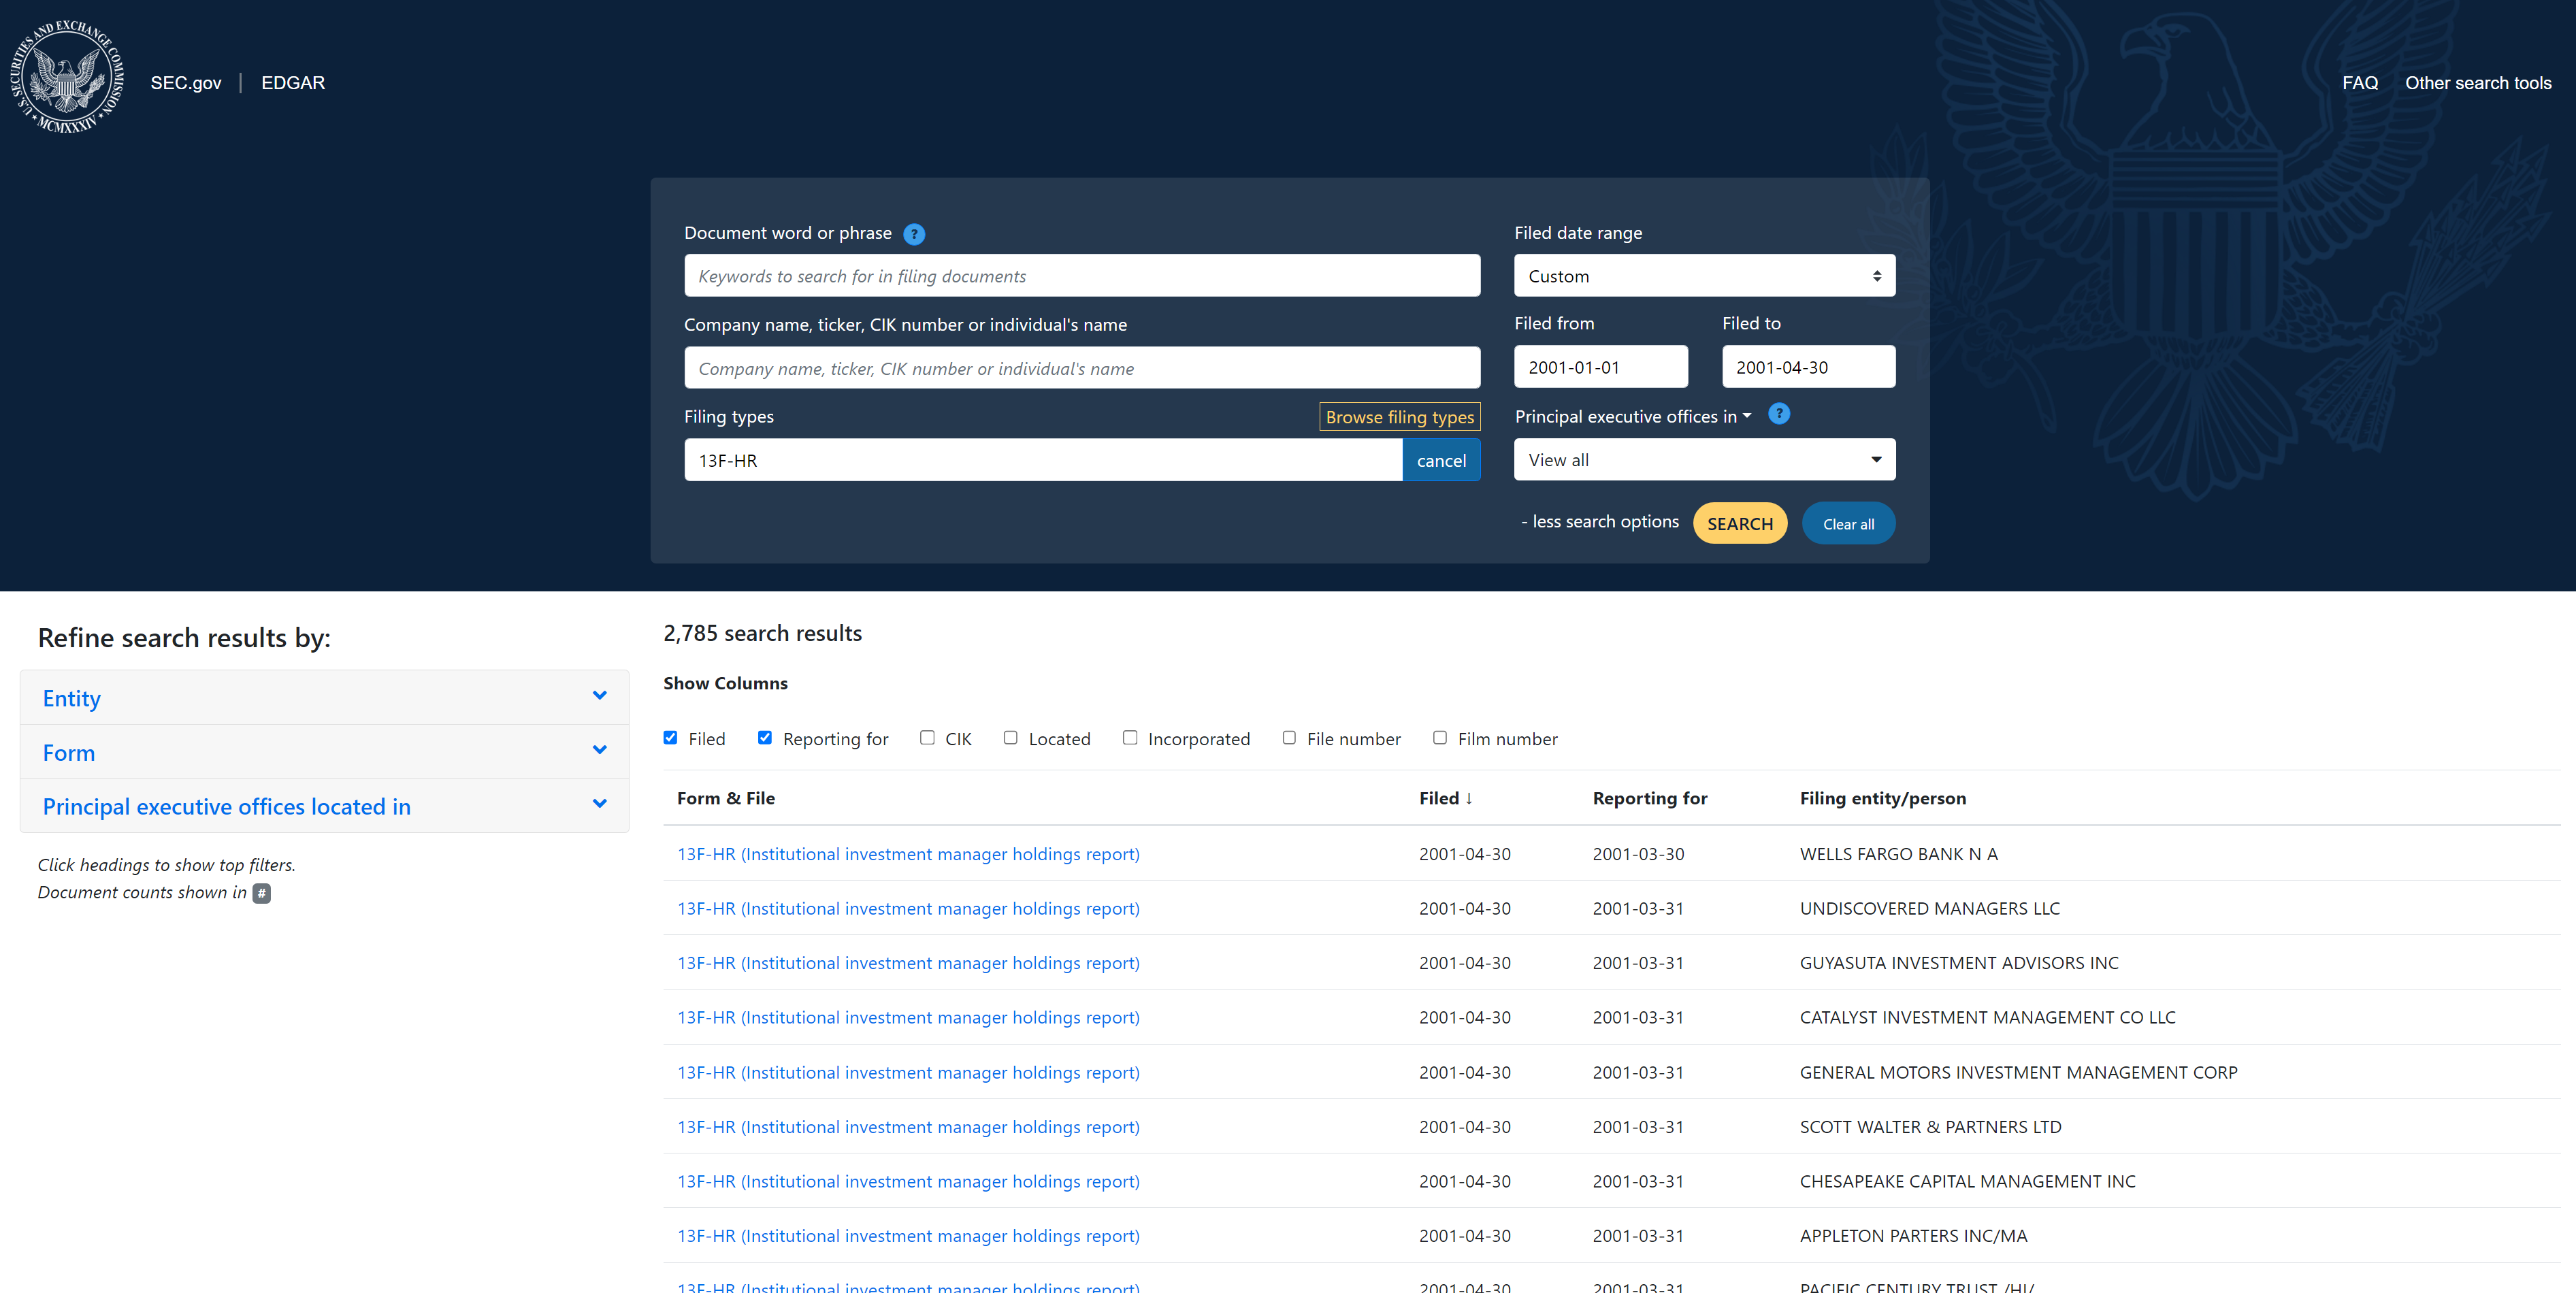
\includegraphics[width=0.8\textwidth]{/POC/data/Scraper_stap1_1.png}
        \caption{Voorbeeld van de bovenkant van resultaatpagina na het uitvoeren van de zoekopdracht.}
        \label{fig:result_s1_1}
    \end{figure}
    
    \begin{figure}[H]
        \centering        
        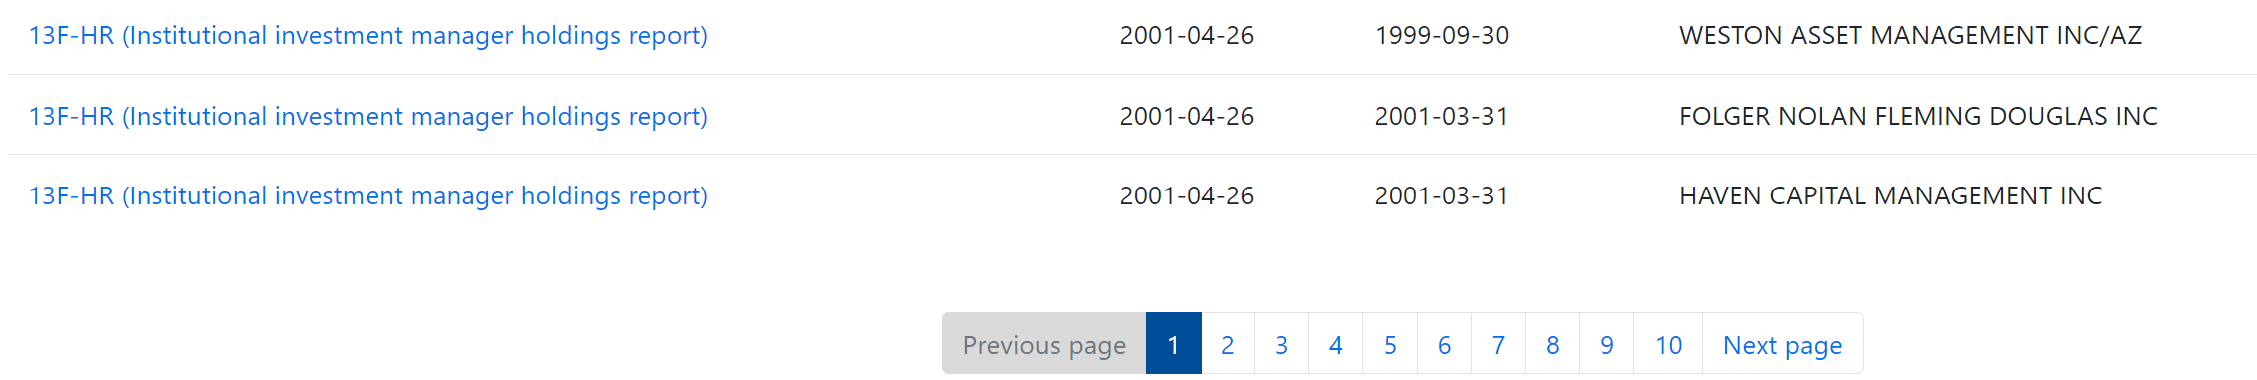
\includegraphics[width=0.8\textwidth]{/POC/data/Scraper_stap1_2.png}
        \caption{Voorbeeld van de onderkant van resultaatpagina na het uitvoeren van de zoekopdracht.}
        \label{fig:result_s1_2}
    \end{figure}
     \textbf{Het resultaat} van deze stap is de resultaatpagina van de query, zoals weergegeven in \autoref{fig:result_s1_1} en \autoref{fig:result_s1_2} , die meerdere pagina's bevat met elk maximaal 100 links naar unieke filings.\\
    \item \textbf{Stap 2:} Op basis van het resultaat van de vorige stap wordt elke link op elke pagina gevolgd, wat resulteert in de weergave van een pop-up (zie \autoref{fig:result_s2_1}) met de details van de filing. Vervolgens wordt op de knop in deze pop-up geklikt om toegang te krijgen tot het overzicht van de gerelateerde bestanden van de filing (zie \autoref{fig:result_s2_2}).\\
    \textbf{Resultaat:} Het resultaat van deze stap is een overzicht van de bestanden die behoren tot de specifieke filing. In dit geval bevat het overzicht slechts twee bestanden, zoals geïllustreerd in \autoref{fig:result_s2_2}.

  
    \begin{figure}[H]
        \centering        
        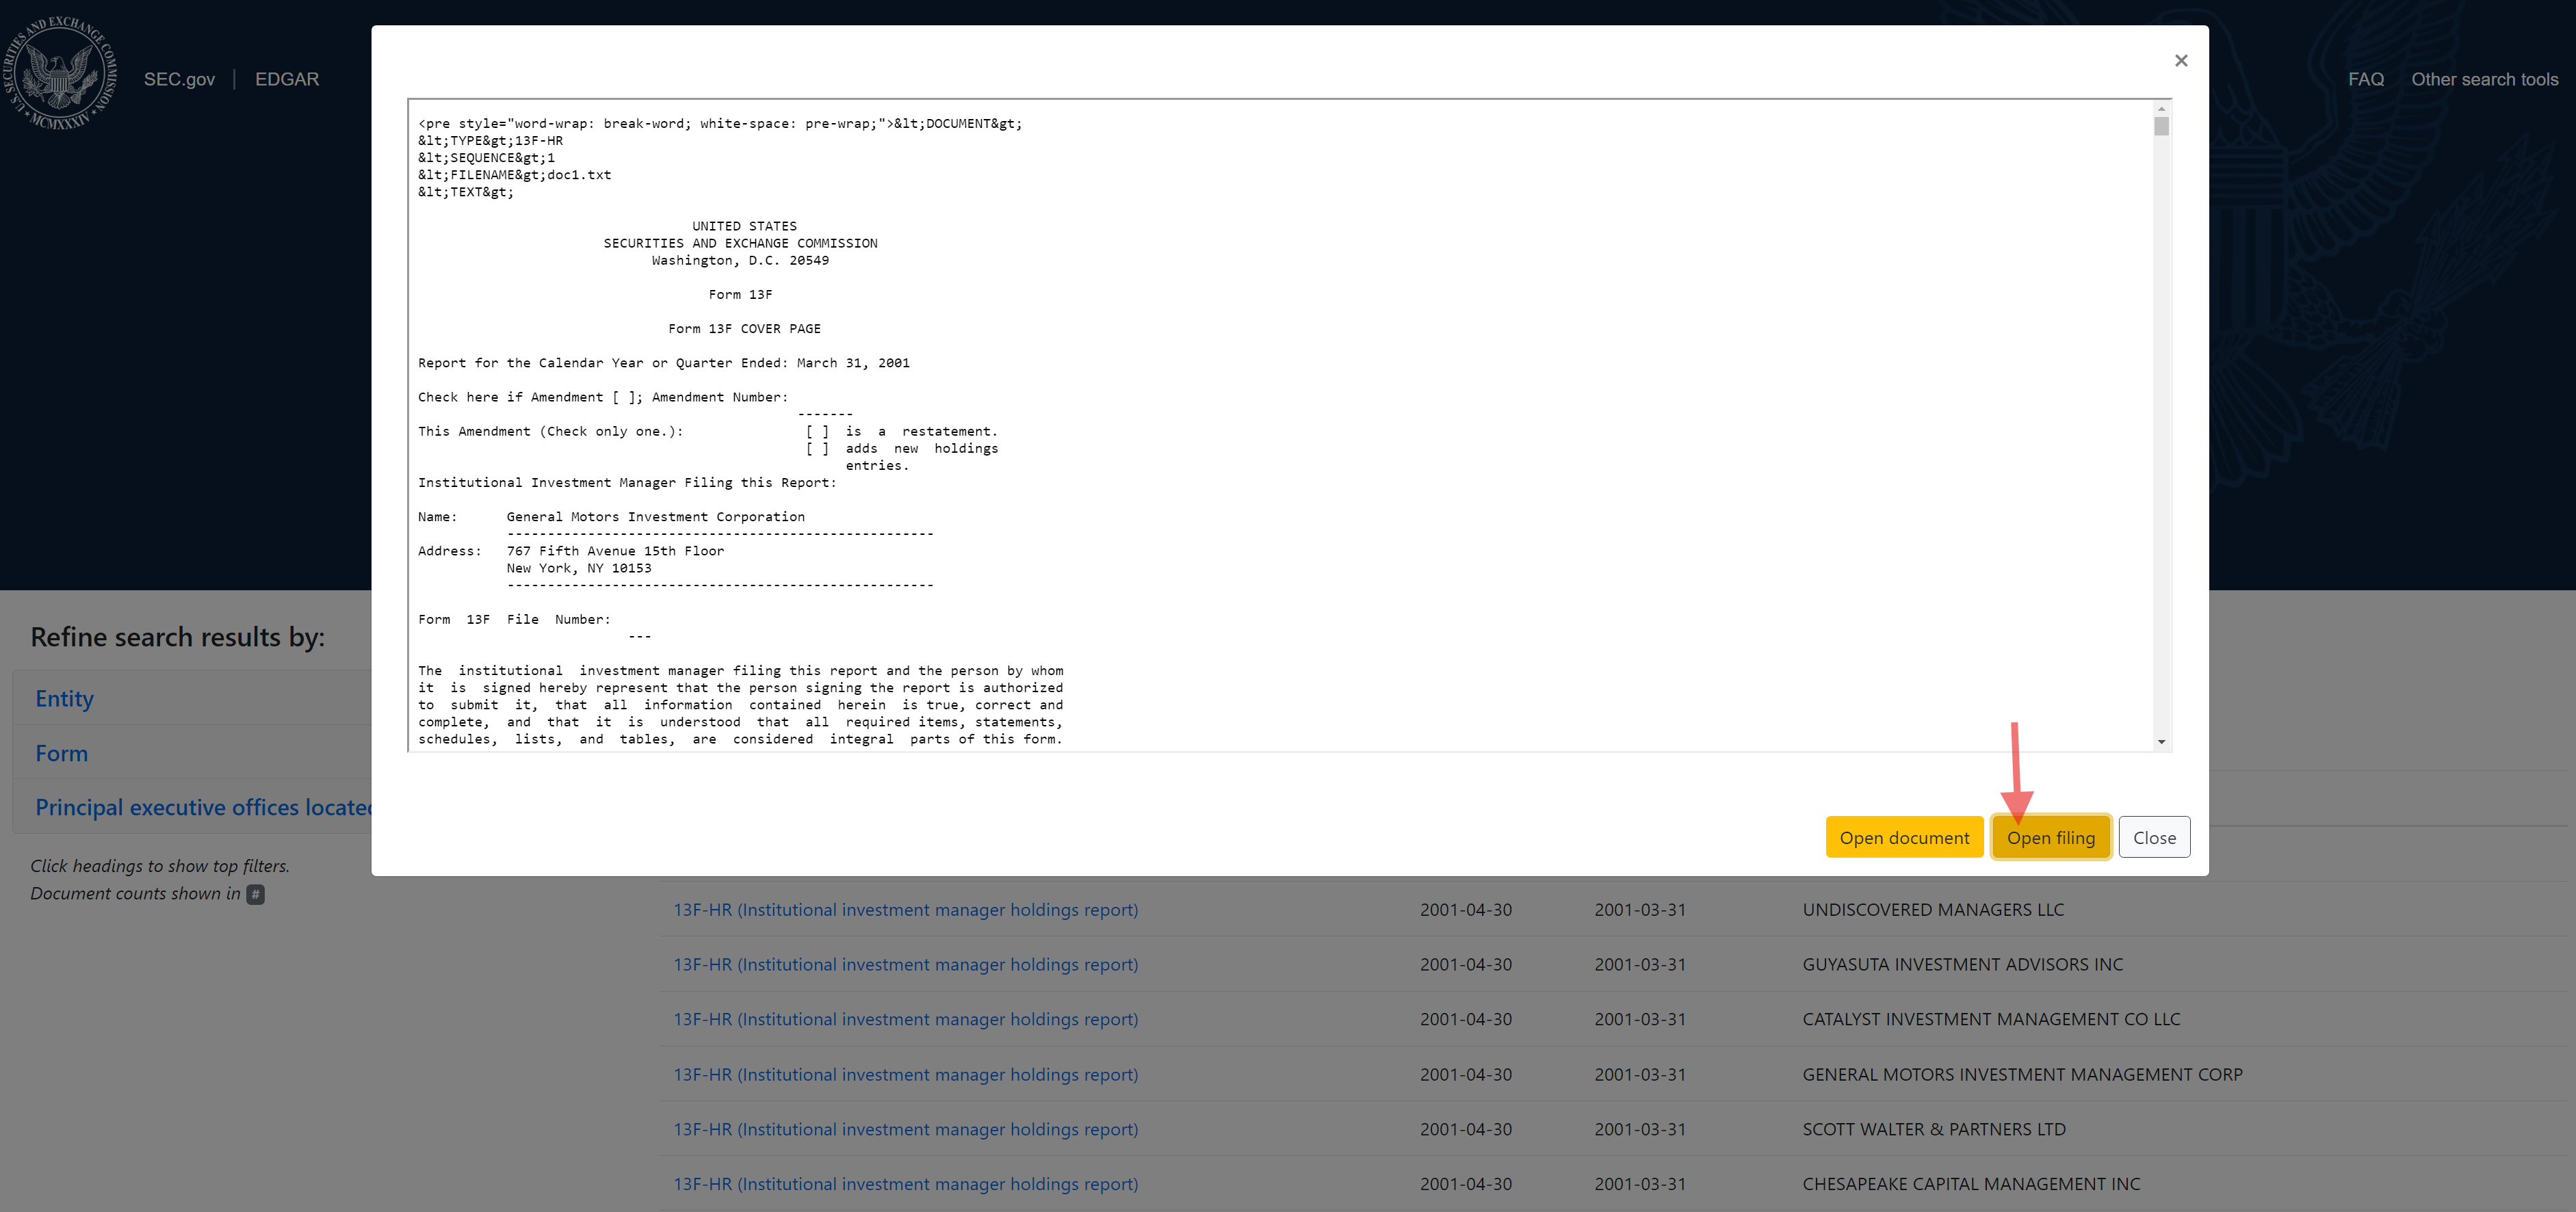
\includegraphics[width=0.8\textwidth]{/POC/data/Scraper_stap2_1.png}
        \caption{Pop-up van een filing.}
        \label{fig:result_s2_1}
    \end{figure}
    
    \begin{figure}[H]
        \centering        
        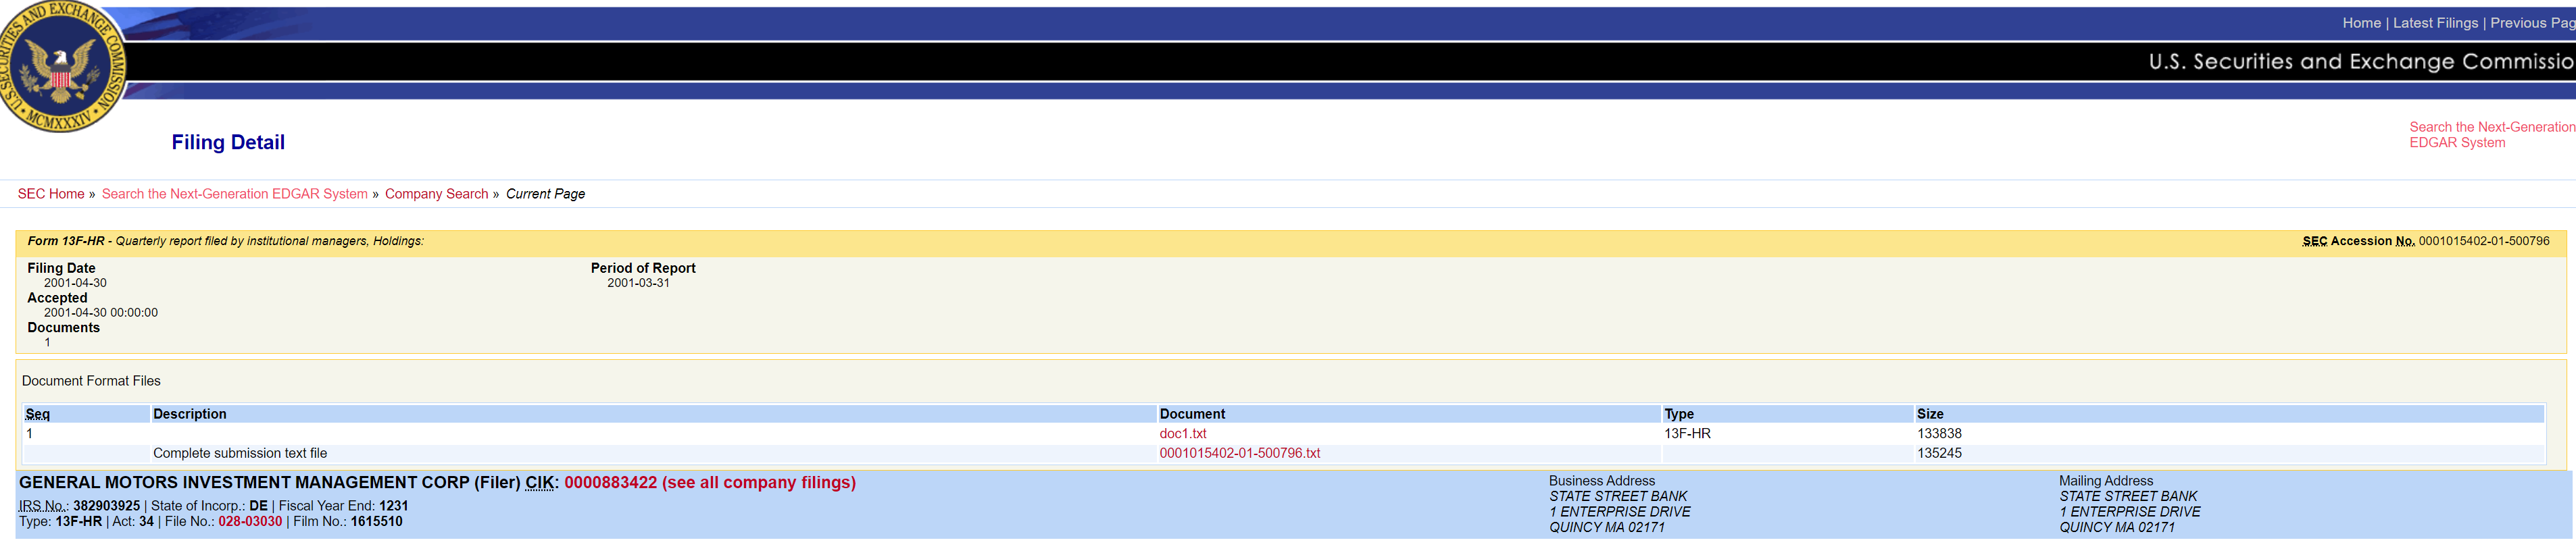
\includegraphics[width=0.8\textwidth]{/POC/data/Scraper_stap2_2.png}
        \caption{Voorbeeld van het overzicht van de bestanden gerelateerd aan één specifieke filing.}
        \label{fig:result_s2_2}
    \end{figure}
    
    \item \textbf{Stap 3:} In deze stap wordt op de link geklikt die de tekst 'Complete submission file' bevat (zie \autoref{fig:Scraper_s3_1}). Door op deze link te klikken, wordt het resulterende bestand gedownload, zoals weergegeven in \autoref{fig:Scraper_s3_2}.
       \begin{figure}[H]
        \centering        
        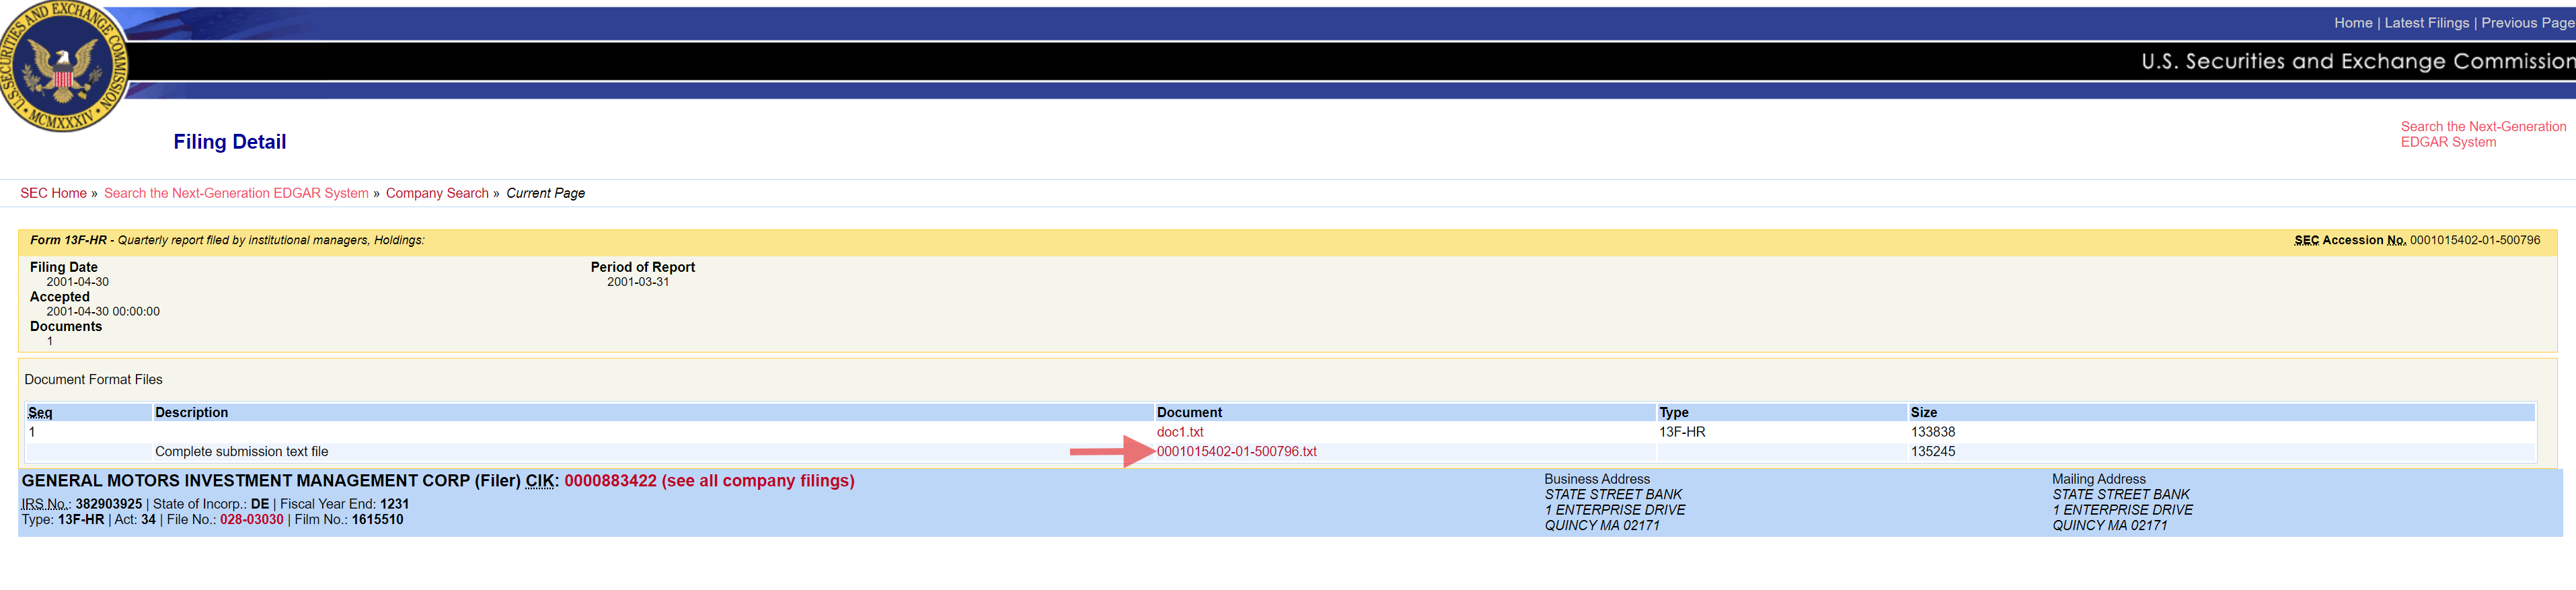
\includegraphics[width=0.8\textwidth]{/POC/data/Scraper_stap3_1.png}
        \caption{Voorbeeld van het overzicht van de bestanden gerelateerd aan één specifieke filing met pijl.}
        \label{fig:result_s3_1}
    \end{figure}
    
    \begin{figure}[H]
        \centering        
        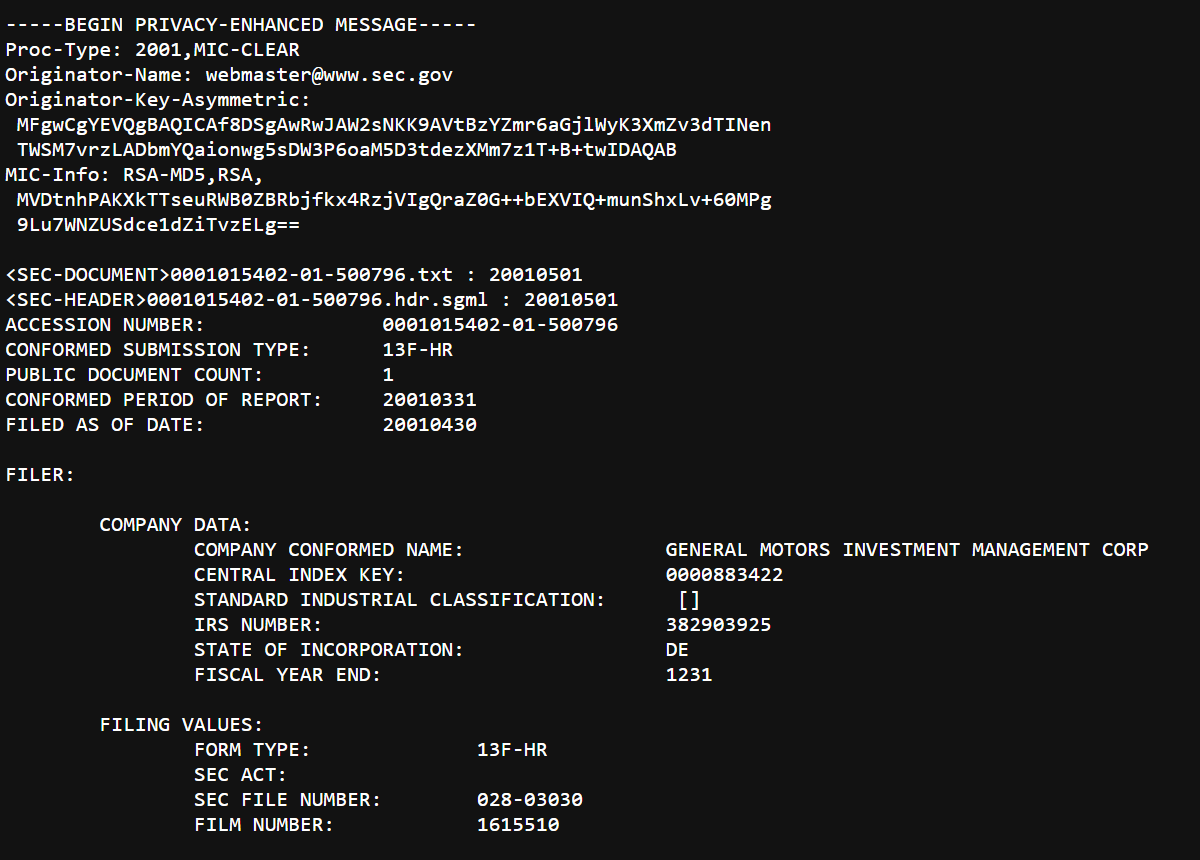
\includegraphics[width=0.8\textwidth]{/POC/data/Scraper_stap3_2.png}
        \caption{Voorbeeld van 13F bestand.}
        \label{fig:result_s3_2}
    \end{figure}
    
\end{enumerate}

\subsection{Data verwerking}
De procedure voor het samenstellen van de dataset begon met het splitsen van de bestanden in twee afzonderlijke componenten: de koptekst \autoref{fig:header} en de tabel \autoref{fig:table_proc} met als essentiële het unieke bestandsnummer. Vervolgens werd het tabelbestand opgeschoond, wat inhield dat HTML-tags werden verwijderd, inzendingen die over meerdere lijnen waren verspreid op een enkele regel werden gezet, lege lijnen werden verwijderd, en het bestandsnummer werd toegevoegd aan de eerste rij van het bestand.

De tabelgegevens werden vervolgens op een methodische manier georganiseerd. Deze gestructureerde tabelgegevens werden, samen met het bijbehorende oorspronkelijke bestand, gebruikt om training sets te genereren. De training set bestond uit twee componenten: het originele (opgeschoonde) bestand \autoref{fig:table_og} en een georganiseerd CSV-bestand \autoref{fig:table_proc} dat de opgeschoonde tabel bevatte. Alsook wordt er een 'Gouden Dataset gemaakt' \autoref{sec:LLMValidation} om het model te kunnen evalueren.  Deze methodologie garandeerde dat de dataset nauwkeurig gestructureerd was, waardoor verdere verwerking, analyse en modellering mogelijk was.

  \begin{figure}[H]
    \centering        
    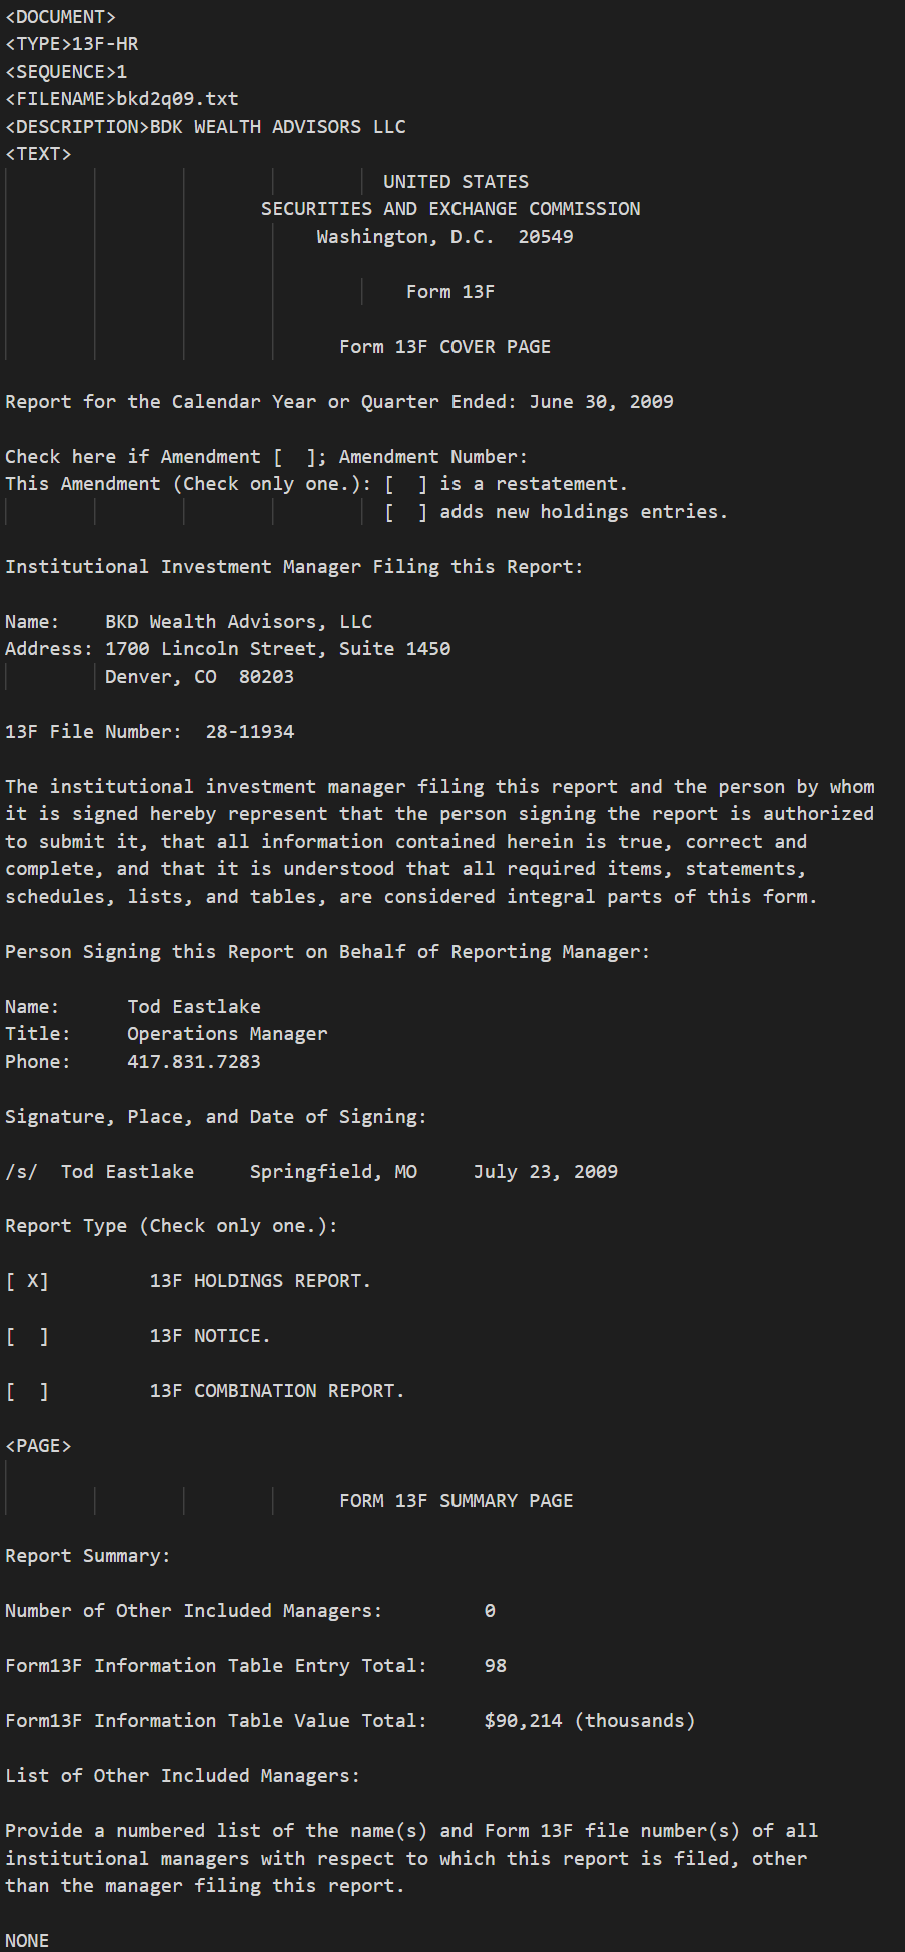
\includegraphics[height=0.8\textheight, keepaspectratio]{/POC/data/header.png}
    \caption{Header van een filing}
    \label{fig:header}
\end{figure}

\begin{figure}[H]
    \centering        
    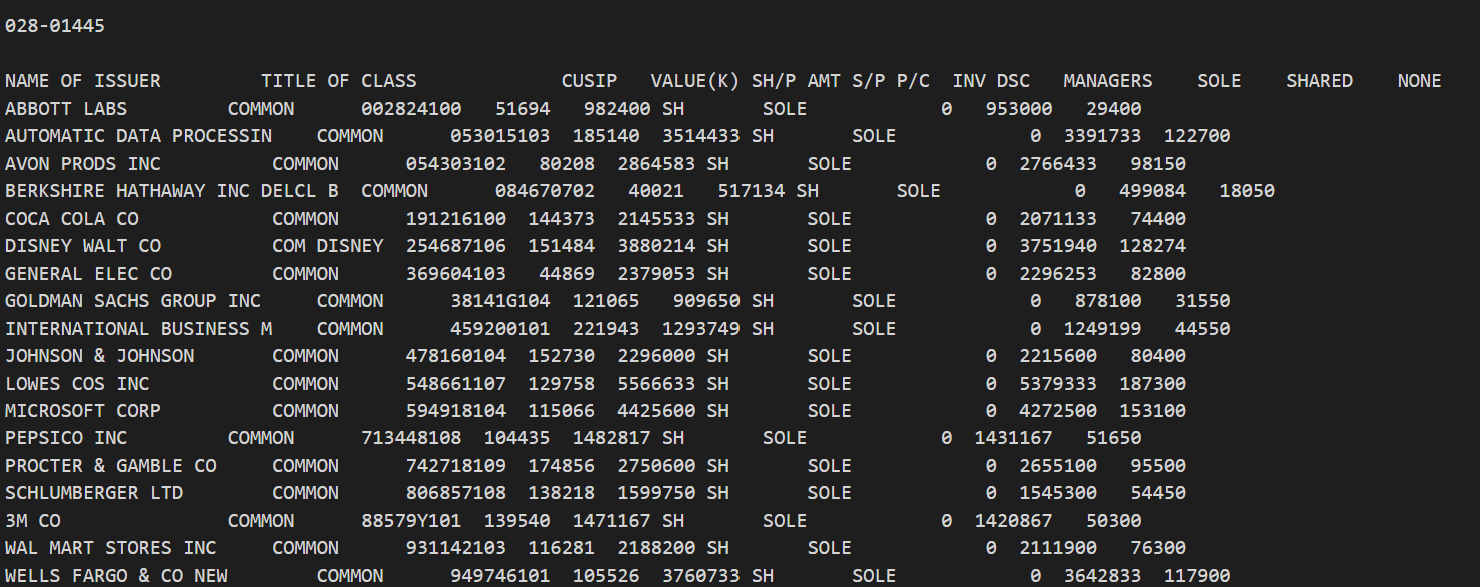
\includegraphics[width=0.8\textwidth]{/POC/data/table_og.png}
    \caption{Voorbeeld van originele tabel van een filing.}
    \label{fig:table_og}
\end{figure}
\begin{figure}[H]
    \centering        
    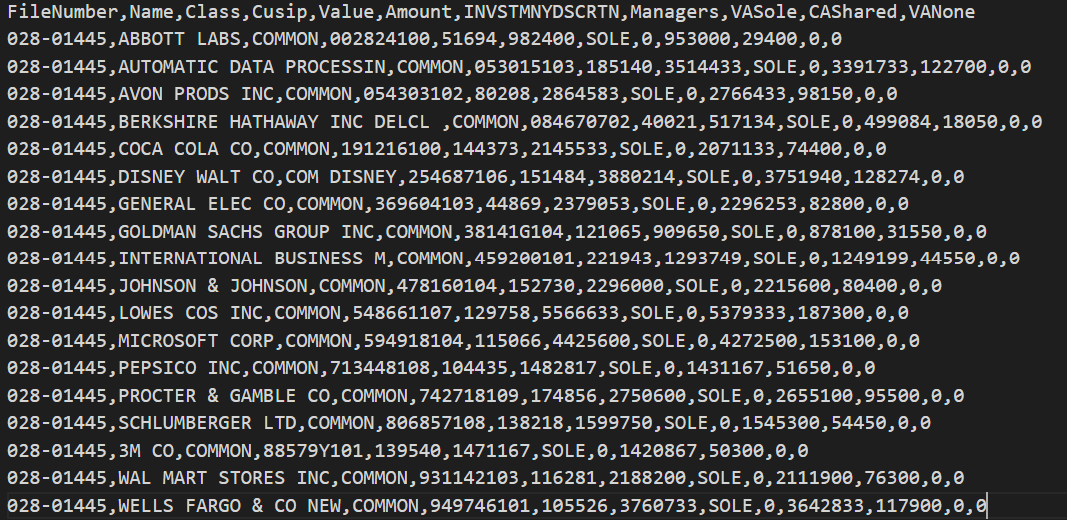
\includegraphics[width=0.8\textwidth]{/POC/data/table_proc.png}
    \caption{Voorbeeld van een verwerkte tabel van een filing.}
    \label{fig:table_proc}
\end{figure}

\subsubsection{Tijdsinschatting dataset creatie}
\label{sec:tijdberekenen}
In deze sectie wordt de benodigde hoeveelheid trainingsdata en de tijd die nodig is om deze te verwerken, berekend. Voor de schatting worden de volgende parameters in overweging genomen:



\begin{enumerate}
    \item \textbf{Verwerkingsduur per filing:} 7 minuten, dit houd in het opkuisen van het bestand maar niets van de data en het opstellen van een correct gekuist bestand en het structureren van de folders.
    \item \textbf{Aantal filings per jaar:} 4
    \item \textbf{Aantal bedrijven (incl. marge):} 510
    \item \textbf{Aantal jaren:} 12
    \item \textbf{Hoeveel percent van originele data}: 0,5\% Zoals vermeld in subsectie: Data vereisten voor LLM's te trainen \ref{sec:DataVereisten} van de literatuurstudie.
\end{enumerate}

\textbf{Het totaal aantal bestanden}, niet meegerekend dat een bedrijf ene dubbelle filing kan doen:
\[
\text{Totaal Aantal Bestanden} = 4 \text{ filings/jaar} \times 505 \text{ bedrijven} \times 12 \text{ jaren} = 24480 \text{ bestanden}
\]
\textbf{Het minimaal aantal bestanden} nodig om een LLM effectieve te trainen:
\[
\text{Minimaal Aantal Bestanden} = 24240 \text{ (Totaal bestanden)} \times 0.005 \text{ (0.5\% van totaal)} \approx 122.4 \text{ bestanden}
\]
\textbf{De totale} tijdsduur voor de verwerking van alle gegevens kan als volgt worden berekend:
\[
\text{Totaal tijd} = \frac{123 \text{ bestanden, afgerond} \times 5 \text{ minuten per bestand}}{60 \text{ minuten per uur}} \approx 14 \text{ uur en}  18 \text{ minuten}
\]

Dit geeft een minimum indicatie van de hoeveelheid tijd die nodig is voor het verwerken van de gegevens voor de hele periode. Dit is essentieel voor het plannen van de benodigde middelen en het vaststellen van de haalbaarheid van het project. Deze berekeningen houd geen rekening met bestanden van voor 2001 sinds deze niet in EDGAR terug te vinden zijn alsook dat er dubbele inzendingen plaats konden gevonden hebben.



\section{Praktische Vergelijking Technieken}
TODO- Expand intro
Llama, Statisticly table extraction, Spacy (IR, IE, NER), REGEX
TODO - show outputs to serve as example and to make it visualy more intresting
Al de technieken zijn gedaan geweest met het zelfde bestand voor zowel de header \autoref{fig:header} als voor de informatie tabel \autoref{fig:table_og}.
\paragraph{Manuele extractie}
Handmatige extractie houdt in dat documenten of bestanden met de hand worden doorgenomen en dat de benodigde informatie wordt overgezet in een gestructureerd formaat, zoals een spreadsheet of een database. Dit proces wordt vaak gebruikt bij kleine datasets of wanneer de gegevens niet beschikbaar zijn in een digitaal formaat.

\begin{enumerate}
    \item \textbf{Voordelen}:
    \begin{enumerate}
        \item Nauwkeurig voor kleine datasets
        \item Simpel
    \end{enumerate}
    \item \textbf{Nadelen}:
    \begin{enumerate}
        \item Niet praktisch voor grote datasets
        \item Tijdrovend
        \item menselijke fouten
        \item Niet schaalbaar
    \end{enumerate}
\end{enumerate}
Vanwege de aard van handmatige extractie is deze niet geschikt voor deze POC, omdat de volledige 13F dataset tienduizenden bestanden bevat.
\textbf{Resultaat}: 
\begin{figure}[H]
    \centering        
    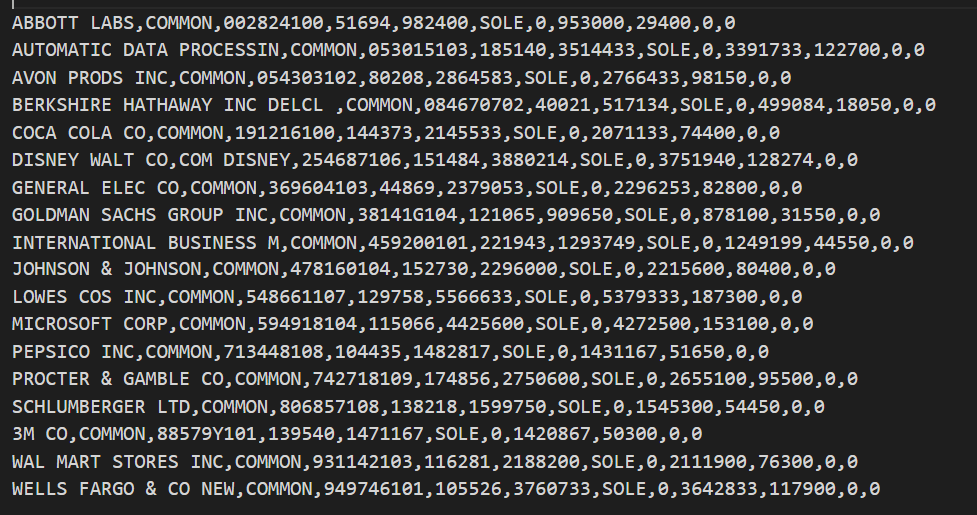
\includegraphics[width=0.8\textwidth]{/POC/data/manual_extraction.png}
    \caption{Voorbeeld van een verwerkte tabel van een filing resulterend van manuele extractie.}
    \label{fig:table_proc}
\end{figure}

\paragraph{REGEX}
Reguliere expressies (regex) zijn patronen die gebruikt worden om opeenvolgingen van tekens in tekst te matchen. Ze kunnen worden gebruikt om specifieke patronen te identificeren en te extraheren uit tekstbestanden, wat bijzonder nuttig kan zijn voor het parsen van gestructureerde of semi-gestructureerde gegevens.
\begin{enumerate}
    \item \textbf{Voordelen}:
    \begin{enumerate}
        \item Flexibel: Regex laat toe om op maat gemaakte patronen maken die passen bij een grote verscheidenheid aan gegevens formaten.
        \item Integratie: Regex is gemakkelijk te integreren in bestaande software
    \end{enumerate}
    \item \textbf{Nadelen}:
    \begin{enumerate}
        \item Complex: naarmate patronen ingewikkelder worden, kan regex moeilijk te lezen en onderhouden beginnen worden.
        \item Gelimiteerd: Regex kan moeite hebben met ongestructureerde of zeer variabele gegevens. Als de gegevens niet voldoen aan een voorspelbaar patroon of als er significante afwijkingen zijn, kan regex niet goed presteren en belangrijke informatie missen of fouten genereren.
    \end{enumerate}
\end{enumerate}

\textbf{Resultaat header}: 
\begin{figure}[H]
    \centering        
    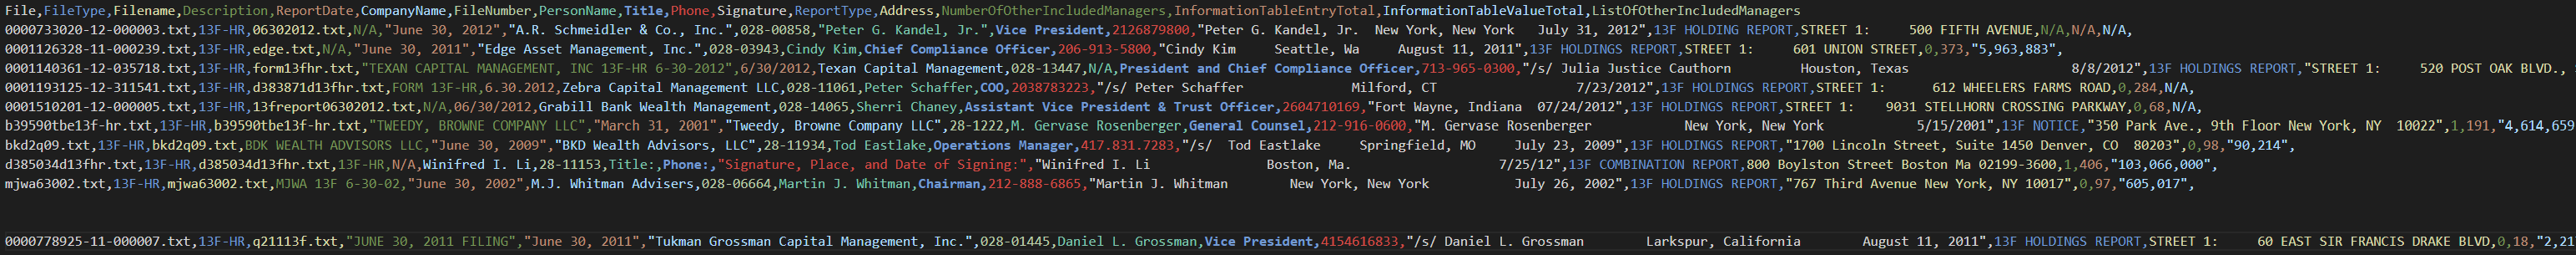
\includegraphics[width=0.8\textwidth]{/POC/data/regex_header.png}
    \caption{Regex header extraction}
    \label{fig:regex header}
\end{figure}
\textbf{Resultaat tabel}: 

Vanwege de aard van de informatie in de 13F-rapportagetabellen bleek het schrijven van een regex aanvankelijk een noodzakelijke stap voor het ontwikkelen van een werkend proof of concept (POC). Bij het extraheren van data uit de tabel werd dit echter al zeer snel complex en niet meer onderhoudbaar en werd aldus stopgezet door de grote variëteit in opmaak en structuur, een missende/extra waarden, indentatie verschillen en extra spaties. Maar het REGEX deed het zeer goed in het extraheren van de data uit de header. Hierdoor werd regex niet gebruikt voor het extraheren van de tabel informatie maar wel voor de algemene informatie van het indienende bedrijf.

%\paragraph{Statistic table extraction}
%
%\begin{enumerate}
%    \item \textbf{Voordelen}:
%    \begin{enumerate}
%        \item Reliable
%    \end{enumerate}
%    \item \textbf{Nadelen}:
%    \begin{enumerate}
%        \item 
%    \end{enumerate}
%\end{enumerate}

\paragraph{IR en IE met Spacy}
Het verschil tussen Information Retrieval en Information Extraction blijkt klein, maar beide methoden hebben moeite om missende data op te vangen. Dit was deels verwacht omdat het model vooral getraind is op gestructureerde data en minder goed kan omgaan met ontbrekende of ongestructureerde informatie. Information Retrieval richt zich op het vinden van relevante informatie op basis van zoektermen, terwijl Information Extraction specifieke entiteiten of relaties uit een tekst haalt. 

Het ontbreken van gegevens kan tot onnauwkeurigheden leiden, wat aangeeft dat aanvullende technieken nodig zijn om nauwkeuriger resultaten te verkrijgen. Het model presteert minder goed wanneer de gegevens inconsistent of onvolledig zijn, wat het belang benadrukt van kwalitatief goede, goed gestructureerde data bij deze methoden. 


\paragraph{NER met Spacy}
Hoewel deze benadering beter presteert dan IR (Information Retrieval) en IE (Information Extraction), is het nog steeds niet voldoende. Named Entity Recognition (NER) ondervindt ook problemen, vooral met ontbrekende gegevens. De tool heeft moeite om correcte entiteiten te identificeren en te extraheren wanneer er data ontbreekt of incompleet is, wat de nauwkeurigheid en effectiviteit van het systeem beïnvloedt. Hierdoor blijft de algehele prestatiesubstantie onder de verwachtingen, en zijn er aanvullende aanpassingen en verbeteringen nodig om de resultaten te optimaliseren.
\paragraph{Llama}
Llama presteerde het beste in vergelijking met alle andere technieken, maar ondervindt nog steeds moeilijkheden wanneer het wordt geconfronteerd met structuren die aanzienlijk afwijken van wat het eerder heeft gezien. Ondanks deze uitdaging, heeft Llama echter wel de capaciteit om effectief om te gaan met ontbrekende waarden. Het systeem kan robuust omgaan met ontbrekende gegevens, maar de prestaties kunnen worden beperkt wanneer het wordt geconfronteerd met ongebruikelijke of radicaal verschillende structuren die het nog niet eerder heeft aangetroffen.

\paragraph{Conclusie}


Na evaluatie van de technieken voor gegevensextractie blijkt dat REGEX en Llama de beste resultaten opleveren voor hun specifieke taken. REGEX is bijzonder effectief gebleken voor het extraheren van gegevens uit headers. Zijn vermogen om op maat gemaakte patronen te herkennen maakt het geschikt voor het accuraat extraheren van header informatie. 

Llama blijkt de meest robuuste keuze voor het extraheren van gegevens uit tabellen. Het kan effectief omgaan met ontbrekende waarden en complexe structuren, wat essentieel is voor de verwerking van de tabellen in deze dataset. Hoewel Llama uitdagingen ondervindt bij ongebruikelijke structuren, biedt het de beste prestaties voor tabellen.

In samenvatting zal REGEX worden ingezet voor header extractie, terwijl Llama zal worden gebruikt voor tabelgegevens. Deze aanpak benut de sterke punten van beide technieken en optimaliseert de efficiëntie van de gegevensverwerking.

\section{Databank}
In dit deel van de POC word de relationele databank ontworpen om de geëxtraheerde gegevens in op te beheren en organiseren. De databank zal bestaan uit 4 tabellen: 'Company', 'Person', 'InformationTabel' en 'GeneralInformation'. Dit schema zal dienen als basis voor gegevensextractie- en beheer.

\begin{figure}[H]
    \centering        
    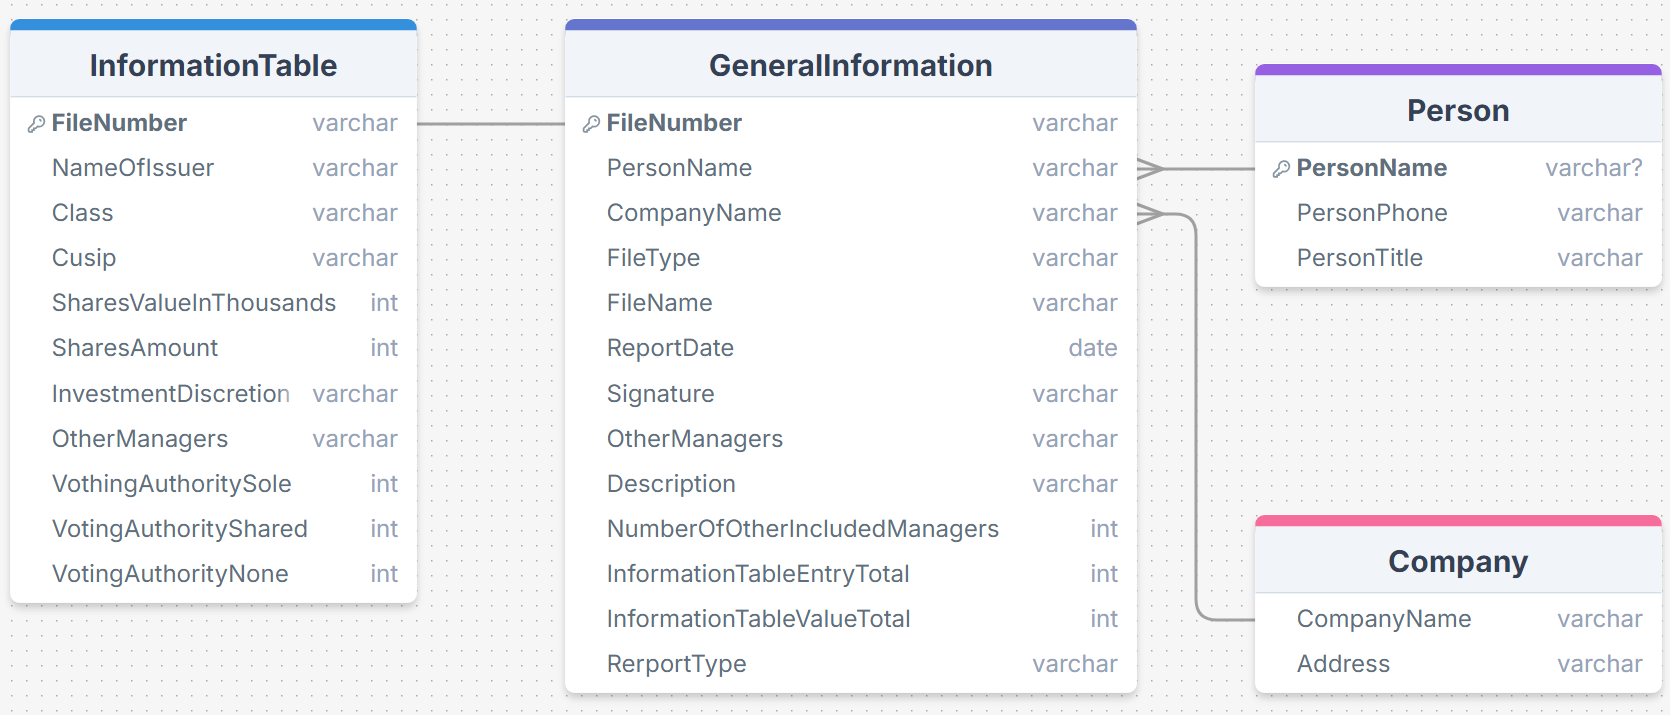
\includegraphics[width=0.8\textwidth]{/POC/db_scheme.png}
    \caption{Databank schema}
    \label{fig:databank_schema}
\end{figure}
\paragraph{'Company' Tabel}

De \textbf{Company} tabel slaat informatie op over verschillende bedrijven. Elke record in deze tabel vertegenwoordigt een afzonderlijk bedrijf.

\begin{enumerate}
    \item \textbf{CompanyName}: De naam van het bedrijf (Primaire Sleutel).
    \item \textbf{Address}: Het adres van het bedrijf.
\end{enumerate}

\paragraph{'Person' Tabel}

De \textbf{Person} tabel bevat gegevens over individuen die zijn gekoppeld aan de bestanden. Elke record vertegenwoordigt een afzonderlijk persoon.

\begin{enumerate}
    \item \textbf{PersonName}: De volledige naam van de persoon (Primaire Sleutel).
    \item \textbf{PersonPhone}: Het telefoonnummer van de persoon.
    \item \textbf{PersonTitle}: De functietitel van de persoon.
\end{enumerate}

\paragraph{'GeneralInformation' Tabel}

De \textbf{GeneralInformation}tabel slaat uitgebreide informatie op die betrekking heeft op elk bestand. Dit omvat details over het bestand zelf, zoals het type, de naam, de handtekening, en aanvullende informatie.


\begin{enumerate}
    \item \textbf{FileNumber}: 13F bestand nummer (Primaire Sleutel).
    \item \textbf{PersonName}: De naam van de persoon die aan het bestand is gekoppeld (Verwijst naar \texttt{Person(PersonName)}).
    \item \textbf{CompanyName}: De naam van het bedrijf dat aan het bestand is gekoppeld (Verwijst naar \texttt{Company(CompanyName)}).
    \item \textbf{FileType}: Het type bestand (13F).
    \item \textbf{FileName}: De naam van het bestand.
    \item \textbf{ReportDate}: De datum waarop het rapport is opgesteld.
    \item \textbf{Signature}: De handtekening op het bestand.
    \item \textbf{OtherManagers}: Beschrijvende tekst over andere managers die aan het bestand zijn gekoppeld.
    \item \textbf{Description}: Een beschrijving van het bestand.
    \item \textbf{NumberOfOtherIncludedManagers}: Het aantal andere managers dat in het bestand is opgenomen.
    \item \textbf{InformationTableEntryTotal}: Het totaal aantal vermeldingen in de informatie tabel.
    \item \textbf{InformationTableValueTotal}: Het totaal van de waarden van de aandelen in de informatie tabel.
    \item \textbf{ReportType}: Het type rapport.
\end{enumerate}

\paragraph{'InformationTable' Tabel}

De \textbf{InformationTable} bevat gedetailleerde informatie over financiële en beheersaspecten die verband houden met elk bestand.


\begin{enumerate}
    \item \textbf{FileNumber}: De unieke identificator voor elk bestand (Verwijst naar \texttt{GeneralInformation(FileNumber)}).
    \item \textbf{NameOfIssuer}: De naam van de uitgever (van de aandelen).
    \item \textbf{Class}: De klasse van de uitgever.
    \item \textbf{Cusip}: Het CUSIP nummer.
    \item \textbf{SharesValueInThousands}: De waarde van de aandelen in duizenden.
    \item \textbf{SharesAmount}: Het aantal aandelen.
    \item \textbf{InvestmentDiscretion}: De investeringsdiscretie.
    \item \textbf{OtherManagers}: Beschrijvende tekst over andere managers.
    \item \textbf{VotingAuthoritySole}: Stemautoriteit uitsluitend.
    \item \textbf{VotingAuthorityShared}: Stemautoriteit gedeeld.
    \item \textbf{VotingAuthorityNone}: Geen stemautoriteit.
\end{enumerate}

\section{Implementatie}
In deze sectie van de proof of concept wordt het proces beschreven voor het extraheren van gegevens uit de 13F-rapporten, zoals eerder besproken in de sectie over gegevensverwerking. De implementatie is verdeeld in drie hoofdsecties: header extractie, tabelextractie, en de invoer in de database.



\subsection{Header data extractie}
De header van elk bestand bevat essentiële informatie, zoals het bestandsnummer, de naam van het bedrijf en andere meta-informatie die cruciaal is voor verdere verwerking en organisatie. Voor de extractie van deze gegevens zijn reguliere expressies (regex) gebruikt, een techniek die bijzonder effectief blijkt te zijn voor het extraheren van gestructureerde informatie uit de headers vanwege het voorspelbare patroon van de informatie.



De eerste stap in dit proces is het identificeren van de relevante metadata. Dit omvat gegevens zoals de naam van het bedrijf, algemene informatie over het bestand en extra details die zich bevinden rondom de informatie tabel. Het zorgvuldig bepalen van deze gegevens is van groot belang om te verzekeren dat alle relevante informatie correct wordt verzameld en verwerkt.

Na het identificeren van de relevante metadata worden patronen voor extractie ontwikkeld door middel van reguliere expressies. Deze patronen zijn zorgvuldig ontworpen om te matchen met de verschillende gegevensvelden die in de header worden verwacht. Het gebruik van regex maakt het mogelijk om flexibel en efficiënt door de tekst te navigeren en specifieke informatie te isoleren op basis van het gestructureerde formaat van de gegevens.



Vervolgens worden de gedefinieerde patronen toegepast op de tekst van de header. De reguliere expressies worden uitgevoerd op elke header tekst om de gegevens te identificeren en te extraheren. Dit proces houdt in dat gezocht wordt naar overeenkomsten in de tekst die voldoen aan de gedefinieerde structuren, wat het mogelijk maakt om snel en nauwkeurig de gewenste informatie te vinden.



Wanneer de regex-patronen overeenkomsten vinden, worden de relevante gegevens uit de tekst gehaald en verzameld. In gevallen waar geen tekstuele overeenkomsten worden gevonden, worden deze gevallen genoteerd als N/A (Not Available). Deze aanpak helpt om een compleet overzicht te krijgen van de gegevens die niet konden worden geëxtraheerd, wat belangrijk is voor latere analyses en correcties.

De verzamelde gegevens worden vervolgens opgeslagen in een CSV-bestand. Dit bestand fungeert als een tussenoplossing en maakt het mogelijk om de gegevens op een gestructureerde manier te bewaren. Later kunnen deze gegevens in bulk naar de databank worden geschreven, waar ze verder kunnen worden verwerkt en geïntegreerd in de bestaande gegevenssystemen. Het gebruik van een CSV-bestand zorgt ervoor dat de gegevens gemakkelijk kunnen worden gecontroleerd en beheerd voordat ze definitief worden overgedragen aan de databank.

Door deze gestructureerde aanpak kan de data-integriteit worden gewaarborgd en kan een efficiënte verwerking van gegevens worden gegarandeerd. Dit draagt uiteindelijk bij aan een beter beheer en een verbeterde toegang tot cruciale informatie.




\subsection{Table data extractie}
\begin{enumerate}
\item \textbf{Voorbereiding van de Trainingsdata}:
    De eerste stap betrof de voorbereiding van de trainingsdata. Hiervoor werden zowel de oorspronkelijke gegevens als de opgeschoonde versies gebruikt. Deze combinatie van datasets biedt een uitgebreid spectrum aan voorbeelden, wat het model helpt om robuust te leren en te generaliseren over verschillende datastijlen en formaten.
\item \textbf{Model Laden}:
Het Llama 3.18B-model werd gedownload vanuit de Unsloth-repository. Tijdens het laden van het model werd de parameter \texttt{params\_max\_seq\_length} ingesteld op basis van de vereiste sequentielengte voor de specifieke data. Deze instelling is cruciaal om ervoor te zorgen dat het model effectief omgaat met de lengte van de inputgegevens.

\item \textbf{Model Initialiseren}:
Na het laden van het model werd het geconfigureerd met de nodige parameters die specifiek zijn afgestemd op de tabel extractietaak. Dit omvatte het afstemmen van hyper parameters en andere instellingen om de prestaties van het model te optimaliseren voor de taak van gegevensextractie.

\item \textbf{Dataset Structureren}:
De dataset werd gestructureerd volgens een format dat lijkt op de Alpaca-prompt. Deze prompt zorgt voor een gestructureerde en herhaalbare manier om instructies, context en verwachte antwoorden te definiëren. Het format is als volgt:

\begin{listing}
    \begin{minted}{python}

    alpaca_prompt = """Hieronder staat een instructie die een taak beschrijft, samen met een invoer die verdere context biedt. Schrijf een antwoord dat de opdracht op de juiste manier voltooit.
    
    ### Instructie:
    {}
    
    ### Invoer:
    {}
    
    ### Reactie:
    {}"""
        \end{minted}
        \caption{Prompt van LLM trainings data}
\end{listing}

Dit formaat helpt om duidelijke en consistente voorbeelden te genereren voor het trainen van het model, wat bijdraagt aan een betere prestaties bij het uitvoeren van de extractietaak.

\item\textbf{ Model Training}:
Het model werd getraind gedurende 30 epochs met een batchgrootte van 2. Tijdens het trainen werd de AdamW-optimalisator met 8-bits precisie gebruikt, met een leerschema ingesteld op 2e-4. Zowel trainings- als validatie sets werden ingezet om de modelprestaties te optimaliseren en over fitting te voorkomen. De training werd zorgvuldig gevolgd om te waarborgen dat het model goed presteerde op zowel bekende als nieuwe data.

\item \textbf{Inferentie Uitvoeren}:
Na de training werd het model opgeslagen voor latere toepassing. Dit betekent dat het model kan worden geladen om inferentie uit te voeren. Tijdens de inferentie wordt het model toegepast op nieuwe gegevens om voorspellingen te doen of gegevens te extraheren op basis van de getrainde kennis.


\item\textbf{ Input Formatteren voor Inferentie}:
De input voor inferentie werd geformatteerd met behulp van de tokenizer volgens het volgende sjabloon:

\begin{listing}
    \begin{minted}{python}
        inputs = tokenizer(
        [
        alpaca_prompt.format(
        "Extraheer de gegevens uit de informatie tabel als CSV", # Instructie
        f"{input}", # Invoer
        "", # Output - laat dit leeg voor generatie!
        )
        ], return_tensors = "pt").to("cuda")
    \end{minted}
    \caption{Prompt voor inference van model}
\end{listing}

Deze formattering zorgt ervoor dat de gegevens correct worden geïnterpreteerd door het model, wat essentieel is voor het verkrijgen van nauwkeurige resultaten.

\item \textbf{Evaluatie van het Model}:
De evaluatie van het model werd uitgevoerd door het gebruik van een gouden dataset, een zorgvuldig samengestelde dataset met een hoge kwaliteit en nauwkeurigheid. Deze gouden dataset fungeerde als een referentie om de prestaties van het model te meten. De resultaten van het model werden vergeleken met deze gouden standaard om te beoordelen hoe goed het model de gegevens kon extraheren en verwerken.

\item \textbf{Resultaten Opslaan}:
De uiteindelijke resultaten van de extractie werden opgeslagen in CSV-bestanden. Elk bestand werd benoemd op basis van het bestandsnummer en opgeslagen in een aangewezen map. Deze gestructureerde aanpak zorgt ervoor dat de resultaten gemakkelijk toegankelijk en controleerbaar zijn voor verdere analyse en rapportage.

\item \textbf{Toevoegen aan de databank: }Na het opslaan van de resultaten werden alle CSV-bestanden in een opgegeven map doorgelopen en toegevoegd aan de database. Dit werd bereikt met behulp van een script dat elke CSV in de map doorloopt, de gegevens inleest en deze gegevens vervolgens naar de database pushte. Het script zorgde ervoor dat alle gegevens op een gestructureerde manier in de database werden opgeslagen, wat de latere toegang en analyse vergemakkelijkte.

\end{enumerate}

\subsection{Resultaten en Beperkingen}

Tijdens het uitvoeren van de bovenstaande stappen kwamen enkele significante uitdagingen naar voren. Vanwege de beperkte tijd en rekenkracht werd slechts een deel van de dataset verwerkt. De resultaten en beperkingen zijn als volgt:

Dataset Voorbereiding:
Het opzetten van een adequaat dataset vereiste een aanzienlijke hoeveelheid tijd, met name het voorbereiden van een representatieve subset van de volledige dataset. Dit proces zou in totaal minstens 15 uur \autoref{sec:tijdberekenen} in beslag nemen. De beperking in beschikbare tijd betekende dat alleen een deel van de volledige dataset werd verwerkt, wat mogelijk invloed heeft gehad op de algehele prestaties en representativiteit van het model.

GPU Vermogen en Trainingstijd:
Het finetunen van het Llama 3.18B-model vereiste net niet meer GPU-kracht dan beschikbaar was, wat resulteerde in een verlengde trainingstijd. De beperkte rekenkracht vertraagde het trainingsproces aanzienlijk, wat het moeilijk maakte om de volledige dataset binnen de beschikbare tijd te verwerken en het model optimaal te finetunen.

Resultaten:
De evaluatie op basis van de gouden dataset toonde aan dat het model goed presteerde bij het extraheren en verwerken van gegevens, maar alleen op data die vergelijkbaar was met de getrainde subset. Het model vertoonde aanzienlijke beperkingen wanneer het werd toegepast op radicaal andere of onbekende data. Deze beperking kan worden toegeschreven aan het feit dat het model voornamelijk is getraind op een beperkte en specifieke subset van gegevens, waardoor de prestaties op afwijkende of nieuwe data minder robuust waren.




\section{Conclusie}
Deze proof of concept (POC) heeft aangetoond dat het gebruik van machine learning-technieken, met name het Llama 3.18B-model, veelbelovend is voor het extraheren van zowel header- als tabelgegevens uit 13F-rapporten. De implementatie omvatte een gestructureerde aanpak waarbij gebruik werd gemaakt van regex voor de header extractie en een getraind model voor tabelextractie. Dit heeft geleid tot een succesvolle en efficiënte gegevensverwerking.

De evaluatie met een gouden dataset heeft bevestigd dat het model in staat is om gegevens met een hoge mate van nauwkeurigheid te extraheren. Ondanks de positieve resultaten zijn er enkele beperkingen vastgesteld. Door tijdsbeperkingen konden niet alle gegevens in de gouden dataset volledig worden verzameld en schoongemaakt. Dit heeft geleid tot een beperkte representativiteit van de gegevens, wat mogelijk invloed heeft gehad op de volledigheid en consistentie van de resultaten.

Desondanks bieden de behaalde resultaten een solide basis voor verdere ontwikkeling en schaalvergroting van deze oplossing. Het model heeft bewezen goed te presteren onder de huidige omstandigheden, en verdere optimalisatie en uitbreiding van de dataset kunnen de nauwkeurigheid en betrouwbaarheid van de extractie verder verbeteren.

In conclusie, hoewel er nog ruimte is voor verbetering, vormt deze POC een belangrijke stap richting het automatiseren van de gegevensverwerking uit financiële rapporten. De ontwikkelde methodologie en modelconfiguratie bieden een veelbelovende oplossing voor het verbeteren van de efficiëntie en nauwkeurigheid van gegevensbeheer in financiële omgevingen. Verdere investeringen in tijd en middelen zullen bijdragen aan het verfijnen van de oplossing en het uitbreiden van de toepassingsmogelijkheden.






\paragraph{Terugkoppeling naar de Onderzoeksvragen}
Hoofdvraag: Het onderzoek heeft bevestigd dat AI-technologieën zoals NLP en ML effectief kunnen worden toegepast om 13F-meldingen te standaardiseren en integreren in een gestructureerde databank. Dit maakt een efficiëntere analyse en vergelijking van historische gegevens mogelijk.
\begin{enumerate}
 \item \textbf{Deelvraag 1: Welke specificaties en uitdagingen zijn verbonden aan 13F-meldingen van de SEC voor 2013?}
 De specificaties en uitdagingen van 13F-meldingen voor 2013, zoals variabele structuren en inconsistenties, vereisten een flexibele aanpak met zowel regex voor headers als ML voor tabellen.

\item \textbf{Deelvraag 2: Hoe kunnen NLP-technologieën worden ingezet om de tekstuele gegevens in 13F-meldingen te extraheren en te standaardiseren?}
NLP-technologieën werden succesvol ingezet om tekstuele gegevens te extraheren en standaardiseren, waarbij regex en een getraind model essentieel waren voor de extractie van gegevens.

 \item \textbf{Deelvraag 3: Wat zijn de praktische implicaties en voordelen van het standaardiseren en integreren van 13F-meldingen met behulp van AI- technologieën?}

 De standaardisatie en integratie van 13F-meldingen met AI-technologieën bieden voordelen zoals verbeterde gegevensstructurering en toegankelijkheid. Ondanks enkele beperkingen, zoals tijdsbeperkingen en rekenkracht, biedt deze aanpak een solide basis voor verdere ontwikkeling.
\end{enumerate}


\paragraph{Beperkingen en Toekomstige Richtingen}
De evaluatie met een gouden dataset heeft bevestigd dat het model in staat is om gegevens met een hoge mate van nauwkeurigheid te extraheren. Er zijn echter enkele beperkingen vastgesteld:
\begin{enumerate}
    \item \textbf{Dataset Voorbereiding}: Het opzetten van een representatieve subset van de volledige dataset vereiste aanzienlijke tijd en middelen. Dit heeft geleid tot een beperkte representativiteit van de gegevens, wat mogelijk invloed heeft gehad op de volledigheid en consistentie van de resultaten.
    
    \item \textbf{GPU Vermogen en Trainingstijd}: De beperkte rekenkracht vertraagde het trainingsproces, wat het moeilijk maakte om de volledige dataset binnen de beschikbare tijd te verwerken en het model optimaal te finetunen.
    
    \item \textbf{Modelprestaties}: Het model vertoonde beperkingen bij het extraheren van gegevens uit radicaal andere of onbekende datastijlen, wat kan worden toegeschreven aan de beperkte subset van getrainde gegevens.
\end{enumerate}

Desondanks bieden de behaalde resultaten een veelbelovende basis voor verdere ontwikkeling. De gestructureerde aanpak en modelconfiguratie vormen een belangrijke stap richting het automatiseren van gegevensverwerking uit financiële rapporten. Verdere optimalisatie en uitbreiding van de dataset kunnen de nauwkeurigheid en betrouwbaarheid van de extractie verbeteren.

In conclusie, hoewel er nog ruimte is voor verbetering, vormt deze POC een essentiële voortgang richting een efficiënter en nauwkeuriger gegevensbeheer in financiële omgevingen. Verdere investeringen in tijd en middelen zullen bijdragen aan het verfijnen van de oplossing en het uitbreiden van de toepassingsmogelijkheden, wat uiteindelijk kan leiden tot een meer robuuste en schaalbare oplossing voor het beheren en analyseren van historische financiële gegevens.